%
% Portuguese-BR vertion
% 
\documentclass{report}

\usepackage{ipprocess}
% Use longtable if you want big tables to split over multiple pages.
% \usepackage{longtable}
\usepackage[utf8]{inputenc} 
\usepackage[brazil]{babel} % Uncomment for portuguese

\sloppy

\graphicspath{{./pictures/}} % Pictures dir
\makeindex
\begin{document}

\DocumentTitle{Documento de Arquitetura}
\Project{ULA}
\Organization{Universidade Estadual de Feira de Santana (UEFS)}
\Version{Build 1.4}

\capa
\newpage
\newpage

%%%%%%%%%%%%%%%%%%%%%%%%%%%%%%%%%%%%%%%%%%%%%%%%%%
%% Revision History
%%%%%%%%%%%%%%%%%%%%%%%%%%%%%%%%%%%%%%%%%%%%%%%%%%
\chapter*{Histórico de Revisões}
  \vspace*{1cm}
  \begin{table}[ht]
    \centering
    \begin{tabular}[pos]{|m{2cm} |m{2cm}| m{6cm} | m{3cm}|} 
      \hline
      \cellcolor[gray]{0.9}
      \textbf{Date} & \cellcolor[gray]{0.9} \textbf{Versão}  &\cellcolor[gray]{0.9}\textbf{Descrição} & \cellcolor[gray]{0.9}\textbf{Autor(s)}\\
      \hline
      8/04/2015 & 1.0 & Concepção e estruturação do Documento & Alexandre Cavalcanti \\ \hline      
      09/04/2015 & 1.1 & \textit{Stakeholders} & Alexandre Cavalcanti \\ \hline
      10/04/2015 & 1.2 & Adição de conteúdo na sessão ULA & Alexandre Cavalcanti \\ \hline      
      11/04/2015 & 1.3 & Datapath & Alexandre Cavalcanti \\ \hline      
      13/04/2015 & 1.4 & Banco de Registradores & Kelvin Carmo, Patrícia Gomes \\ \hline
      15/04/2015 & 1.5 & Conclusão dos tópicos e revisão & Alexandre Cavalcanti \\ \hline      
    \end{tabular}
  \end{table}

% TOC instantiation
\tableofcontents

%%%%%%%%%%%%%%%%%%%%%%%%%%%%%%%%%%%%%%%%%%%%%%%%%%
%% Document main content
%%%%%%%%%%%%%%%%%%%%%%%%%%%%%%%%%%%%%%%%%%%%%%%%%%
\chapter{Introdução}
  
  \section{Propósito do Documento}
  Este documento descreve a implementação de uma unidade lógica aritmética e de um banco de registradores, elementos que compõe a arquitetura de um processador de uso comum, incluindo especificações dos circuitos internos, além do datapath do sistema. O documento apresenta também os módulos funcionais e como eles interagem entre si, assim como as definições de entradas e saídas.Serão detalhados os elementos utilizados na arquitetura, assim como as motivações que levaram a tais escolhas e a influência destes elementos no produto final.
  
  \section{Stakeholders}
    \FloatBarrier
    \begin{table}[H] 
      \begin{center}
        \begin{tabular}[pos]{|m{6cm} | m{8cm}|} 
          \hline 
          \cellcolor[gray]{0.9}\textbf{Nome} & \cellcolor[gray]{0.9}\textbf{Papel/Responsabilidades} \\ \hline
          Alexandre Cavalcanti, Fábio Barros, Jhone Mendes, Jussara Machado, Kelvin Carmo, Lucas Morais, Patricia Gomes, Pedro Mota & Desenvolvimento\\ \hline
          Fábio Barros, Jhone Mendes, Jussara Machado, Lucas Morais, Pedro Mota & Implementação\\ \hline
          & Testes\\ \hline
          Alexandre Cavalcanti, Kelvin Carmo & Confecção da documentação\\ \hline
        \end{tabular}
      \end{center}
    \end{table} 

\section{Visão Geral do Documento}

O presente documento é apresentado como segue:

\begin{itemize}
  
  \item Sessão 2 - Apresenta uma visão geral sobre a ULA,banco de registradores e banco de flags, abordando questões como, função determinada no sistema.
  \item Sessão 3 - Descreve detalhadamente a arquitetura, explanando os módulos e componentes do projeto, explicando e citando suas restrições.
  \item Sessão 4 - Descreve o funcionamento básico do sistema de controle.

\end{itemize}

  % inicio das definições do documento
  \section{Definições}
    \FloatBarrier
    \begin{table}[H]
      \begin{center}
        \begin{tabular}[pos]{|m{5cm} | m{9cm}|} 
          \hline
          \cellcolor[gray]{0.9}\textbf{Termo} & \cellcolor[gray]{0.9}\textbf{Descrição} \\ \hline
          Datapath & Caminho de dados percorrido para a execução de uma instrução. \\ \hline
          Overflow & Quando um determinado valor a ser representado ultrapassa a quantidade de bits disponíveis na ULA \\ \hline         
        \end{tabular}
      \end{center}
    \end{table}  
  % fim

  % inicio da tabela de acronimos e abreviacoes do documento
  \section{Acrônimos e Abreviações}
    \FloatBarrier
    \begin{table}[H]
      \begin{center}
        \begin{tabular}[pos]{|m{2cm} | m{12cm}|} 
          \hline
          \cellcolor[gray]{0.9}\textbf{Sigla} & \cellcolor[gray]{0.9}\textbf{Descrição} \\ \hline
            ULA & Unidade Lógica Aritmética \\ \hline
        \end{tabular}
      \end{center}
    \end{table}  
  % fim

\chapter{Visão Geral}
\section{ULA}

    A unidade Lógica Aritmética(ULA) é um circuito combinatório responsável por realizar operações aritméticas e lógicas dentro de um processador. As operações a serem executadas são determinadas através dos sinais de controle recebidos pela ULA em sua entrada de operação. Logo após os dados de entrada são computados e o resultado é obtido na saída do circuito.
    
    
\paragraph{}
    A complexidade da ULA é proporcional à complexidade do sistema em que será utilizada, assim, como o propósito é desenvolver uma ULA que irá atuar num processador de uso geral, utilizaremos uma ULA simples, contendo operandos de 2bytes, podendo assim representar números de -128 até 127.A ULA tbm é capaz de decidir através do resultado da operação a ocorrência de flags. Essas são:
    
    \begin{itemize}
    \item ZERO : Flag que sinaliza se o resultado da operação é 0;
    \item CARRY : Flag que indica se há um "vai-um" para fora do Bit Mais Significativo;
    \item SIGNED : Flag que indica se o resultado da operação é negativo ou positivo;
    \item OVERFLOW : Flag que indica que o resultado da operação excede a representção máxima de números do sistema;
    \end{itemize}

\begin{figure}[H] \centering 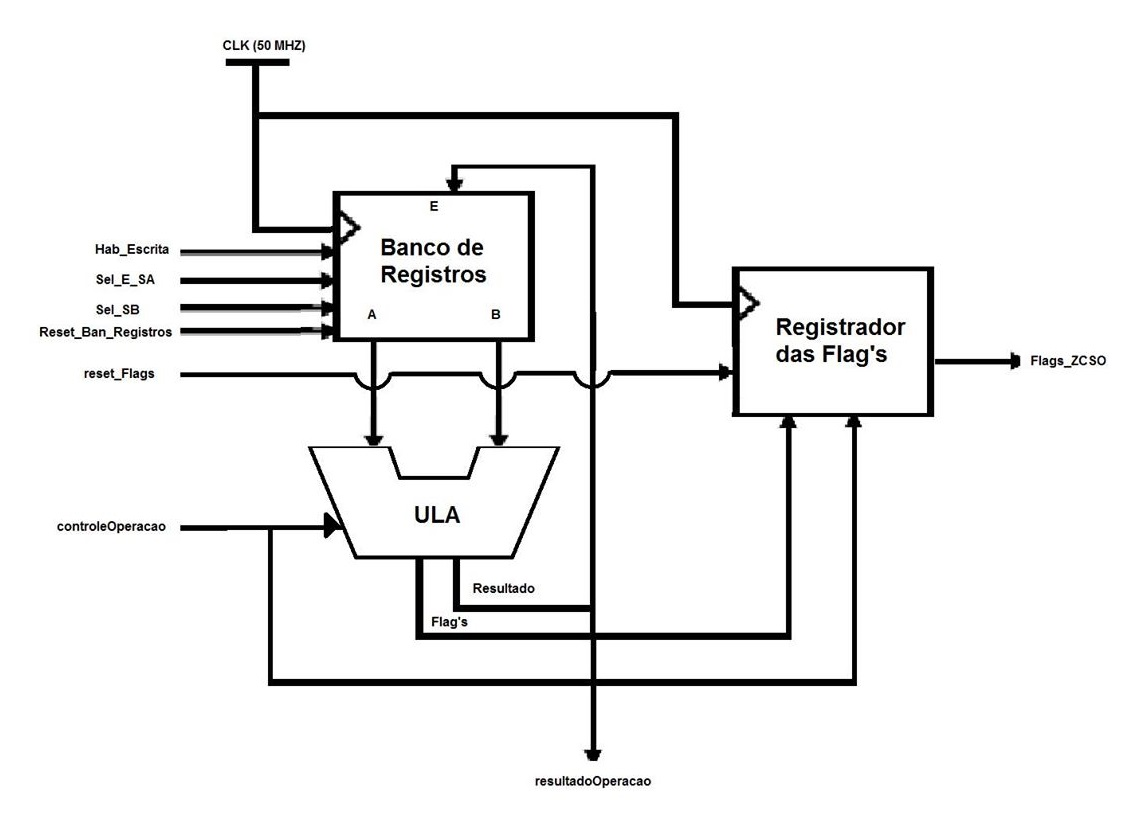
\includegraphics[width=0.9\textwidth]{datapathrs123.png}                \caption{Datapath ULA} \label{fig:mesh1} 
    \end{figure}

\paragraph{}
    A ULA deve possuir comportamento semelhante ao da tabela abaixo:
        \begin{table}[H] 
      \begin{center}
        \begin{tabular}[pos]{|m{2cm} | m{4cm}| m{3cm}| m{3.5cm}|} 
          \hline 
          \cellcolor[gray]{0.9}\textbf{Código} & \cellcolor[gray]{0.9}\textbf{Operação} & \cellcolor[gray]{0.9}\textbf{Mnemônico} & \cellcolor[gray]{0.9}\textbf{Flags Atualizadas} \\ \hline
00000 & C = A + B & add c, a, b & todas\\ \hline
00001 & C = A + B + 1 & addinc, c, a, b & todas\\ \hline
00011 & C = A + 1 & inca c, a & todas\\ \hline
00100 & C = A – B – 1 & subdec c, a, b & todas\\ \hline
00101 & C = A – B & sub c, a, b & todas\\ \hline
00110 & C = A – 1 & deca c, a & todas\\ \hline
01000 & C = Deslocamento Lógico Esq. (A) & lsl c, a & S, C, Z\\ \hline
01001 & C = Deslocamento Aritmético Dir. (A) & asr c, a & S, C, Z\\ \hline
10000 & C = 0 & zeros c & nenhuma\\ \hline
10001 & C = A.B & and c,a,b & Z, S\\ \hline
10010 & C = !A.B & andnota c, a, b & Z, S\\ \hline
10011 & C = B & passb c, a & nenhuma\\ \hline
10100 & C = A.!B & andnotb c, a, b & Z, S\\ \hline
10101 & C = A & passa, c, a & Z, S\\ \hline
10110 & C = A & xor B xor c, a, b & Z, S\\ \hline
10111 & C = A | B & or c, a, b & Z, S\\ \hline
11000 & C = !A.!B & nand c, a, b & Z, S\\ \hline
11001 & C = !(A xor B) & xnor c, a, b & Z, S\\ \hline
11010 & C = !A & passnota c, a & Z, S\\ \hline
11011 & C = !A|B & ornota c, a, b & Z, S\\ \hline
11100 & C = !B & passnotb c, b & Z, S\\ \hline
11101 & C = A|!B & ornotb c, a, b & Z, S\\ \hline
11110 & C = !A|!B & nor c, a, b & Z, S\\ \hline
11111 & C = 1 & ones c & nenhuma\\ \hline
          
    \end{tabular}
    \end{center}
    \end{table}
    
\section{Banco de Registradores}
O banco de registradores é onde os dados que serão manipulados estarão salvos, sujeitos a alterações futuras. Inicialmente o banco de registradores possui 3 registradores, os dois primeiros para os operandos e o terceiro para o resultado da operação . Cada registrador possui a capacidade de armazenamento de 16 bits e para endereçá-los foram usados 2 bits, sendo possível dessa forma o endereçamento de até 4 registradores.


\subsection{Registradores de Estado ( Flags )}
São registradores responsáveis por sinalizar um determinado acontecimento inesperado após a execução de uma operação.Esse bloco recebe da ULA os sinais necessários para a ativação das flags necessárias.



\chapter{Especificações Técnicas}
    \section{ULA}
    \paragraph{} 
    Segue abaixo uma representação em bloco da ULA, com suas respectivas entradas e saídas para uma visualização mais dedicada e explicativa sobre o módulo. 
    
    \begin{figure}[H] \centering \includegraphics[width=0.9\textwidth]{ULA.jpeg}                \caption{Datapath ULA; Z = ZERO, C = CARRY, S = SIGNED, O = OVERFLOW} \label{fig:mesh1} 
    \end{figure}
    
    \subsection{Entradas}
\begin{itemize}
\item $operandoA$ $e$ $operandoB$: Duas entradas de 16 bits, responsáveis por receber dos registradores A e B os dados referentes aos operandos.
\item $controle$ : Entrada de 5 bits para controle de operação.
\end{itemize}


    \subsection{Saídas}
\begin{itemize}
\item $resultadoOp$ : Saída de 16 bits, através da qual o resultado da operação realizada será salvo no banco de registradores;
\item $Z$, $C$, $S$ $e$ $O$ : 4 Saídas de 1 bit que será enviado para o Banco de registrador de flags para ativação das flags necessárias; 
\end{itemize}

    \section{Banco de Registradores}
    \paragraph{} 
    Segue abaixo uma representação em bloco do Banco de Registradores, com suas respectivas entradas e saídas para uma visualização mais dedicada e explicativa sobre o módulo. 
    
    \begin{figure}[H] \centering \includegraphics[width=0.9\textwidth]{banco_de_registradores.jpeg}                \caption{Datapath Banco de Registradores} \label{fig:mesh1} 
    \end{figure}
    \subsection{Entradas}
\begin{itemize}
        \item $Sel_SA$ (2 bits): Entrada do endereço do primeiro registrador que será lido;
		\item $Sel_SB$ (2 bits): Entrada do endereço do segundo registrador que será lido;
		\item $Sel_SC$ (2 bits): Entrada do endereço do registrador de destino, para 					armazenar um resultado da ULA;
		\item $dado_escrita$ (8 bits): Entrada do dado que será armazenado no registrador de 				resultado especificado pelo endereço em $Sel_SC$.
\end{itemize}

\subsection{Saídas}
\begin{itemize}
\item $A$ (8 bits): Saída do dado do registrador especificado pelo endereço $address_RegA$;
\item $B$ (8 bits): Saída do dado do registrador especificado pelo endereço $address_RegB$.
\end{itemize}

\subsection{Sinais de Controle}
\begin{itemize}
\item $HabEscrita$ (1 bit): Sinal para controle da escrita dos registradores, seu estado é baixo para manter o mesmo dado no registrador até que uma instrução termine de ser executada, o mesmo pode ser alterado para alto, apenas quando uma escrita de dados for necessária;
\item $clock$: Entrada de clock;
\item $reset$: Sinal de reset. Zera todos os dados contidos nos registradores;
\end{itemize}
    
\section{Registradores de Flags}
    \paragraph{} 
    Segue abaixo uma representação em bloco do Registradores de Flags, com suas respectivas entradas e saídas para uma visualização mais dedicada e explicativa sobre o módulo. 
    
    \begin{figure}[H] \centering \includegraphics[width=0.9\textwidth]{reg_flags.jpeg}                \caption{Datapath Banco de Registradores de Flags} \label{fig:mesh1} 
    \end{figure}
    
    \subsection{Entradas}
\begin{itemize}
        \item $controleOperacao$ (5 bits): Entrada do controle de operação da ULA, que serve para determinar ao registrador quais flags devem ser atualizadas dependendo da operação realizada;
		\item $Z$, $C$, $S$ $e$ $O$ (2 bits): Entradas de 1 bit , vindas da ULA , com os valores das flags(ZERO, CARRY, SIGNED, E OVERFLOW) atualizadas a depender da operação;
\end{itemize}

\subsection{Saídas}
\begin{itemize}
\item $ZCSO$ (4 bits): Saída das 4 flags finalmente atualizadas;
\end{itemize}

\subsection{Sinais de Controle}
\begin{itemize}
\item $clock$: Entrada de clock;
\item $reset$: Sinal de reset. Zera todos os dados contidos nos registradores;
\end{itemize}
% Optional bibliography section
% To use bibliograpy, first provide the ipprocess.bib file on the root folder.
% \bibliographystyle{ieeetr}
% \bibliography{ipprocess}

\end{document}
